%        File: problema4_1.tex
%     Created: Wed Nov 18 10:00 AM 2015 A
% Last Change: Wed Nov 18 10:00 AM 2015 A
%
\documentclass[a4paper]{report}
\usepackage[english]{babel}
\usepackage{enumitem}
\usepackage{mathrsfs}
\usepackage{amsmath}
\newcommand\norm[1]{\left\lVert#1\right\rVert}
\usepackage{graphicx}
\graphicspath{ {images/} }

\begin{document}
\begin{enumerate}[label=\emph{\alph*)}]
  \item %a) What is the order of magnitude of differential accelerations caused by individual perturbations in LEO? What are the most relevant perturbations? How do things change in GEO?
    For LEO, the order of magnitud of the \textbf{differential} accelerations are:
    \begin{itemize}
      \item Spherical Earth = $10^0$
      \item J2 = $10^{-2}$
      \item J3 = $10^{-5}$
      \item Moon = $10^{-7}$
      \item Sun = $10^{-7}$
      \item Solar Radiation Pressure(100\%) = $10^{-8}$
      \item Solar Radiation Pressure(2\%) = $10^{-10}$
    \end{itemize}
    For GEO orbits, Moon, Sun, and Solar Pressure terms remain almost the same, and Spherical Earth, J2 and J3 terms are reduce by a magnitude of $10^{-2}$.

  \item % b) How do we include Earth’s oblateness J 2 perturbations in the relative dynamics model? What are the secular effects of J2 perturbations on the relative orbit elements (ROE)? Show these effects geometrically in ROE space
    In order to include J2 effects, we only take its long-term and secular effects. Neglecting second order effects, we can write the variation of ROE as a function of the relative excentricity and inclination vectors $\delta \vec{i}$ and $\delta \vec{e}$, and the chief's orbit inclination $i$:

    \[\dot{\delta\alpha} = \left( \begin{array}{c}
      0 \\
      -\frac{21}{2}\gamma n \sin{2i} \delta i_x \\
      -\frac{3}{2}\gamma n(5\cos{i}^2-1) \delta e_y \\
      \frac{3}{2}\gamma n (5\cos{i}^2)\delta e_x \\
      0 \\
      3\gamma\sin{i}^2 \delta i_x
      \end{array} \right) \]   
    Integrating this equation over $u$, we get:
    \[\delta \alpha(t) = \left( \begin{array}{c} \delta a \\ \delta \lambda - \frac{21}{2}(\gamma\sin{2i}\delta i_x + \frac{1}{7}\delta a)(u(t)-u_0) \\ \delta e \cos{\varphi+\varphi'(u(t)-u_0)} \\  \delta e \sin{\varphi+\varphi'(u(t)-u_0)} \\ \delta i_x \\ \delta i_y + 3\gamma \sin{i}^2 \delta i_x (u(t)-u_0) \end{array} \right) \]
    \[\mathrm{with}~~\varphi' = \frac{d\varphi}{du} = \frac{3}{2} \gamma (5 \cos{i}^2-1) \]

    Analysing the result, we se that J2 does no affect $\delta e$ magnitud, but its phase $\phi$. The normalized speed of this variation depends mainly of the inclination $i$. Looking at the inclination vector, we see that only $i_y$ is afected by $J_2$ being its effect positive for the for $+\delta i$ and negative for $-\delta i$. Finally, looking the $\delta a, \delta \lambda$ plane, we se $J_2$ effects only $\delta\lambda$, depending on the relative inclination $\delta i$ and obsolute inclination $i$. $i$ can be chosen in order to produce an exactly oposite displacement than the one produce by Kepler due to $\delta a != 0$, in order to keep a $\delta a$ value without changing $\delta \lambda$.
  
  \item % c) How much does the relative eccentricity vector rotate in 15 days in LEO? For which inclinations is the motion counter-clockwise? At what inclinations is the J 2 effect removed?
    Assuming that the chief's orbit inclination is $i = 55^o$ and the excentricity $e = 0$, the value of $\varphi'$ is $0.00030016$. For a LEO orbit ($h = 500 km$), the orbit period is of 1.57 hs, this means that in 15 days the spacecrafts orbits 228 times. In degrees, this is a value of $u$ of $1436.6~rad$. This means a $24.7^o$ variation of $\varphi$. For $i = 20^o $, $\Delta\varphi = 130^0$.

  \item % e) How much does the relative inclination vector translate in 15 days in LEO? For which inclinations is the motion “upwards”? At what inclinations is the J2 effect removed? Can we remove this effect by a proper selection of the ROE?
    Making the same assumption done in \textit{c)}, and a relative inclination $\delta i_x=5^o$, $\delta i_y$ augments acording to $\Delta \delta_y = 3\gamma\sin{i\cdot\delta i_x}^2\cdot\Delta u = 0.805^o $. The motion is ´´upwards´´ for values of $i > 0^o$. For equatorial orbits J2 effects disapear. The same happens when the relative inclination is $i_x = 0$.
   
  \item % f) How much does the relative mean longitude translate in 15 days in LEO due to Kepler and J2 effects? At what inclinations is the J2 effect removed? Can we obtain bounded relative motion in the presence of J2 effects by a proper selection of the ROE?
    J2 effects appear in presence of $\delta i_x$, while keplerian effects appear in presence of a relative semi-mayor axis $\delta a$ (the conmensurability condition is no longer satisfy). For 15 days LEO orbit with $\delta i_x = 5^o$ and $\delta a = 0.2\cdot10^{-3}$ (1.5 km diference), the relative mean longitud $\delta\lambda$ translates $-66^o$ due to J2 and $-18^o$ due to $\delta a$. J2 effects can be remove either in equatorial orbits or polar orbits, and also by setting the relative inclination $\delta i_x$ to $0$. Bounded relative orbits ($\delta \lambda = 0$) can be obtain even in presence of J2 efects by setting the Kepler effect to be oposite to J2 effects. For the current example, this meas a relative semi-mayor axis $\delta a = -0.53\cdot10^{-3}$ (deputy orbit's semi-mayor axis is $3.67~km$ smaller than chief obit's semi-mayor axis). 

  \item % g) What are the relevant secular effects caused by differential drag on the ROE? Show these effects geometrically in ROE space. How well can we match the ballistic coefficients of two spacecraft in LEO (use GRACE as example)? Can we neglect differential drag for closely flying identical spacecraft? When is your conclusion no longer valid?
    The relevant secular efects due to differential drag on th ROE are:
    \begin{figure}[h]
      \begin{minipage}{0.5\textwidth}
	\[ \delta \lambda(t) = \frac{3}{8an^2} \Delta B \rho v^2 (u(t)-u_0)^2\]
	\[ \delta a(t) = -\frac{1}{2an^2}\Delta B \rho v^2(u(t)-u_0)\]
      \end{minipage}
      \begin{minipage}{0.5\textwidth}
         \centering
         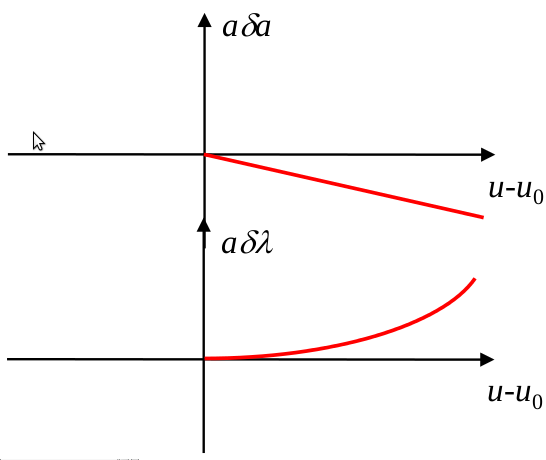
\includegraphics[width=\textwidth]{secular_drag_effects}
      \end{minipage}
    \end{figure}
    Where $v$ is the chief spacecraft's speed, $\rho$ is the density, and $\Delta B$ is the relative ballistic coefficient ($B = cd~ A/m$). The ballistic coeficient can be match to roughly $1\%$ at launch, with another $1\%$ variation during lifetime due to differential fuel consumption. This means, for LEO orbits, differential acceleration of $<10 nm/s^2$. This effects can be neglected except in the presence of safe modes or non-cooperative spacecraft (different in deputy's and chief's attitude producing different $cd$).


  \item % h) How can we incorporate impulsive maneuvers in the relative dynamics model? How can we derive closed-form deterministic impulsive maneuvering schemes? Summarize the effects of impulsive maneuvers in R, T, and N
    Impusive maneuvers can be expressed in terms of the ROE by inversion of the solution of the HCW equations, obtaining:
    \[ \begin{array}{r c c c}
      \delta a \approx & & 2 \delta v_t/(na) & \\    
      \delta \lambda \approx & -2\delta v_r/(na) & -3(u-u_M)\delta v_t/(na) & \\
      \delta e_x \approx & \delta v_r \sin{u_M}/(na) & +2\delta v_t\cos{u_M}/(na) & \\
      \delta e_y \approx & -\delta v_r \cos{u_M}/(na) & +2\delta v_t \sin{u_M}/{na} & \\
      \delta i_x \approx & & & +\delta v_n \cos{u_M}/(na) \\
      \delta i_y \approx & & & +\delta v_n \sin{u_M}/(na) 
  \end{array}\]
  where $(\delta v_r,\delta v_t,\delta v_n)$ is the relative velocity obtain with the impulsive maneuvers expresed in the chief's RTN frame. We can see that the out-of-plane maneuver is decoupled from the along-track and radial maneuvers. A close form solution can be obtain by dividing the in-plane maneuver in two seperate maneuvers.


  \item % i) Why do we aim at closed-form solution of the relative motion control problem?
    Close form solutions allow us to plan maneuvers for formation keeping over the mission lifetime or to acquire new formation geometries.

  \item % j) Describe the closed-form minimum delta-v solution for out-of-plane control, both geometrically and analytically
    For out-of-plane maneuver, the $\delta v_n$ required and the maneuvre location $u_M$ in order to mantain a require $\vec{\delta i}^{man}$ are:
    \begin{figure}[h]
      \begin{minipage}{0.5\textwidth}
	\[\delta v_n = n a \norm{\vec{\delta i}^{man}-\vec{\delta i}} \]
	\[ u_M = \tan{\frac{\vec{\delta i_y}^{man}-\vec{\delta i_y}}{\vec{\delta i_x}^{man}-\vec{\delta i_x}}}^{-1} \]
	where $\vec{\delta i}$ is the current inclination vector. In the case of correcting J2 effects, only $\delta i_y$ varies, so the maneuver position is $u_M = \pi$.
      \end{minipage}
      \begin{minipage}{0.5\textwidth}
	\centering
	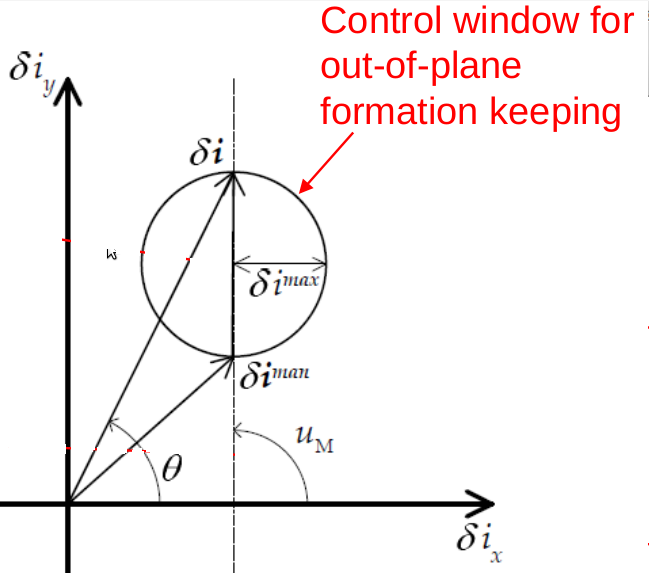
\includegraphics[width=\textwidth]{Out-of-plane_maneuvre}
      \end{minipage}
    \end{figure}

  \item % k) Describe the closed-form minimum delta-v solution for in-plane control (two pulses), both geometrically and analytically
    For in plane formation keeping, the minimum $\delta v$ two impulse solution consists in two along-track impulses separated $180^o$ in mean argument of latitud (radial impulses are less eficient). The maneuver corrects both $\delta a$ (in order to mantain a bouded orbit) and $\vec{\delta e}$:\\
    \begin{figure}[h]
    \begin{minipage}{0.5\textwidth}
      \[\delta {v_t}_1 = \frac{n a}{4} \left[ (\delta a^{man} - \delta a) + \norm{\delta e^{man} - \delta e} \right] \]
      \[\delta {v_t}_2 = \frac{n a}{4} [(\delta a^{man} - \delta a) - \norm{\delta e^{man} - \delta e}] \]
      \[{u_M}_1 = \tan{\frac{(\delta e_y^{man}-\delta e_y)}{(\delta e_x^{man} - \delta e_x)}}^{-1} \]
      \[{u_M}_2 = {u_M}_1 + \pi \]
    \end{minipage}
    \begin{minipage}{0.5\textwidth}
	\centering
	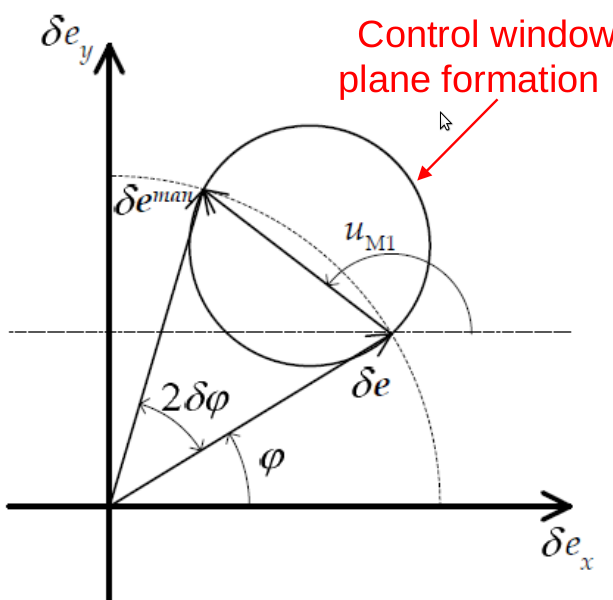
\includegraphics[width=\textwidth]{In-plane_maneuvre}
    \end{minipage}
  \end{figure}

  \item % l) Describe the closed-form minimum delta-v solution for in-plane control (three pulses), both geometrically and analytically

  \item % m) Describe how we try to generalize the closed-form solution approach for large reconfigurations including perturbations

\end{enumerate}
\end{document}



